% This is the main tex file
% Please leave the following settings unchanged!
% ___________________________________________________________________
\documentclass{scrartcl}%


\usepackage{amsmath}%
\usepackage{amsfonts}%
\usepackage{amssymb}%
\usepackage{graphicx}
\usepackage{geometry}
\usepackage{hyperref}
\usepackage{color}
\usepackage{caption}
\usepackage{ngerman} 
\usepackage[utf8]{inputenc}
\usepackage{tabularx}
\usepackage{longtable}
\usepackage{colortbl}
\usepackage{float}
\usepackage{xcolor}
\usepackage[onehalfspacing]{setspace}
\usepackage{graphicx}
\usepackage{url}


%  Definition of some mathematical environments
\newtheorem{theorem}{Theorem}
\newtheorem{acknowledgement}[theorem]{Acknowledgement}
\newtheorem{algorithm}[theorem]{Algorithm}
\newtheorem{axiom}[theorem]{Axiom}
\newtheorem{case}[theorem]{Case}
\newtheorem{claim}[theorem]{Claim}
\newtheorem{conclusion}[theorem]{Conclusion}
\newtheorem{condition}[theorem]{Condition}
\newtheorem{conjecture}[theorem]{Conjecture}
\newtheorem{corollary}[theorem]{Corollary}
\newtheorem{criterion}[theorem]{Criterion}
\newtheorem{definition}[theorem]{Definition}
\newtheorem{example}[theorem]{Example}
\newtheorem{exercise}[theorem]{Exercise}
\newtheorem{lemma}[theorem]{Lemma}
\newtheorem{notation}[theorem]{Notation}
\newtheorem{problem}[theorem]{Problem}
\newtheorem{proposition}[theorem]{Proposition}
\newtheorem{remark}[theorem]{Remark}
\newtheorem{solution}[theorem]{Solution}
\newtheorem{summary}[theorem]{Summary}
\newenvironment{proof}[1][Proof]{\textbf{#1.} }{\ \rule{0.5em}{0.5em}}

\parindent 0.0mm
\geometry{a4paper,left=30mm,right=25mm, top=25mm, bottom=2cm}

% ___________________________________________________________________
% ___________________________________________________________________


\begin{document}
	\title{Softwarepraktikum: \\ 
		Implementierung eines Tools zur forensischen Analyse von ShellBags unter Windows 10}
	\author{Conny Karras und Anna-Lena Totzauer
		\\
		\\ \small{Cybercrime/Cybersecurity, CY19wC-M}
		\\ \small{Betreuer: Prof. Dr. rer. nat. Labudde}
		\\ \small{Bearbeitungszeitraum: April 2020 - Juli 2020}
		\\ \footnotesize{}}

   	\date{}
	\maketitle
 	\thispagestyle{empty}

	 \newpage 
	 \tableofcontents
	 \thispagestyle{empty}
	
	 \newpage
	 \pagenumbering{Roman}
	 \listoffigures
	 \addcontentsline{toc}{section}{Abbildungsverzeichnis}
	 
	 \listoftables
	 \addcontentsline{toc}{section}{Tabellenverzeichnis}
	 \newpage
	 
	 \pagenumbering{arabic}

	
	
	% Aufgabenstellung und Motivation
	\section{Aufgabenstellung und Motivation}
\vspace{0.5cm}
Dr. Edmund Locards Austauschprinzip \glqq Every contact leaves a trace\grqq{} wurde ursprünglich für die reale Welt formuliert. Doch auch in der digitalen Welt hinterlassen Aktivitäten Spuren auf einem System. Hierbei werden unter anderem Einträge in der Windows-Registry vorgenommen. \cite[S.5]{carvey2011windows} 

Die sogenannten ShellBags sind ein Teil dieser Registrierungsdatenbank. Sie speichern zum einen Einstellungen wie Fenstergröße, -position und Ansichtseinstellungen, zum anderen wird ein Eintrag abgelegt, sobald ein Ordner erstellt und geöffnet wurde. \cite[S.26]{kavrestad2018fundamentals} 

Welche Informationen die ShellBag-Registrierungsschlüssel speichern und wie sie aufgebaut und im Klartext zu verstehen sind, wurde bereits in der Bachelorarbeit von Anna-Lena Totzauer zum Thema \glqq Forensische Analyse von Windows ShellBags\grqq{} genauer untersucht. Basierend auf dieser Arbeit soll nun im Rahmen eines Softwarepraktikums ein Tool entwickelt werden, welches eine forensische Live-Analyse von ShellBags unter Windows 10 ermöglicht. Dafür sollen die in der Registry enthaltenen Informationen in einer für den Menschen unmittelbar lesbaren Form dargestellt werden. Darüber hinaus soll es möglich sein, die gefundenen Einträge zu exportieren. Mithilfe dieses Tools soll die Analyse der ShellBags erleichtert werden, da sie so nicht mehr händisch ausgelesen werden müssen. Dies führt auch zu einer Vermeidung von menschlichen Fehlern.  Darüber hinaus können die gewonnenen Informationen durch einen Export gesichert werden. \newline
Nachfolgend werden zunächst die theoretischen Grundlagen für ShellBags unter Windows 10 aufgegriffen. Darauf folgen die Qualitätsanforderungen an das Tool, Informationen zur praktischen Umsetzung, eine Bedienungsanleitung sowie die Validierung des Tools. Im Anschluss erfolgt eine Diskussion darüber, ob das Tool die zuvor festgelegten Qualitätsanforderungen erfüllt und was gegebenenfalls hätte optimiert werden können. Die beiden darauffolgenden Kapitel beinhalten ein zusammenfassendes Fazit sowie einen Ausblick. 


	%Zielsetzung, Motivation
	
	% Grundlagen ShellBags
	\section{Theoretische Grundlagen}
\vspace{0.5cm}
Nachfolgend werden die Grundlagen für ShellBags erläutert, welche für die Implementierung des Tools notwendig sind. Es handelt sich somit nur um einen Auszug der für das Projekt wichtigsten Grundlagen. 

\subsection{Allgemeines}
\vspace{0.3cm}
Die ShellBag-Schlüssel sind ein Teil der Windows-Registrierungsdatenbank, kurz Registry genannt, welche Konfigurationsdaten des Betriebssystems und seinen Programmen sowie Benutzereinstellungen speichert \cite[S.215]{anson2012mastering}. Die Registry besteht aus fünf Root Keys, von denen zwei als Master Keys bezeichnet werden, die tatsächlich physisch in der Registry abgelegt sind. Die anderen drei Keys sind nur abgeleitet von Schlüsseln unter den beiden Master Keys und somit nur Spiegelungen. \cite[S.219]{anson2012mastering} 
\newpage
Die fünf Root Keys werden nachfolgend erläutert:
\begin{itemize}
	\item \texttt{HKEY\_LOCAL\_MACHINE} ist ein Master Key und wird somit nicht von anderen Keys abgeleitet. Dieser Key enthält Konfigurationsdaten des Computers.
	\item \texttt{HKEY\_USERS} ist ebenfalls ein Master Key. Dieser Key enthält Informationen über alle Benutzer, die jemals im System eingeloggt waren.
	\item  \texttt{HKEY\_CURRENT\_USER} ist abgeleitet von einem Schlüssel unter HKU. Er enthält die Einstellungen des aktuell angemeldeten Benutzers.
	\item \texttt{HKEY\_CLASSES\_ROOT} ist dafür zuständig, dass zu einem bestimmten Dateityp das richtige Programm ausgewählt wird. Dieser Schlüssel wird abgeleitet aus HKLM und HKCU.
	\item \texttt{HKEY\_CURRENT\_CONFIG} enthält Konfigurationseinstellungen der Hardware und wird abgeleitet von HKLM. \cite[S.219]{anson2012mastering}
\end{itemize}
Im Registrierungs-Editor werden die Keys genau in dieser Form dargestellt, allerdings werden die Informationen physisch gesehen in verschiedene Dateien, den sogenannten Hives, ausgelagert. Die Informationen werden somit nicht so zentral und zusammenhängend wie im Registrierungs-Editor, sondern über die gesamte Festplatte verteilt abgelegt. \cite[S.220]{anson2012mastering} 

Wo diese Hives tatsächlich auf der Festplatte abgelegt sind, erfährt man unter \texttt{HKEY\_LOCAL\_MA- \newline CHINE$\backslash$SYSTEM$\backslash$CurrentControlSet$\backslash$Control$\backslash$hivelist}. Wenn das System die Hives in die Registry laden will, wird in diesem Key geprüft, wo die Dateien abgelegt sind. \cite[S.225]{anson2012mastering} \\
\\
Unter Windows 10 werden die ShellBag-Schlüssel unter den folgenden nutzerspezifischen Hives abgelegt: 
\begin{itemize}
	\item \texttt{NTUSER.dat$\backslash$Software$\backslash$Microsoft$\backslash$Windows$\backslash$Shell$\backslash$BagMRU}
	\item \texttt{NTUSER.dat$\backslash$Software$\backslash$Microsoft$\backslash$Windows$\backslash$Shell$\backslash$Bags}
	\item \texttt{USRCLASS.dat$\backslash$Local Settings$\backslash$Software$\backslash$Microsoft$\backslash$Windows$\backslash$Shell$\backslash$ \newline BagMRU}
	\item \texttt{USRCLASS.dat$\backslash$Local Settings$\backslash$Software$\backslash$Microsoft$\backslash$Windows$\backslash$Shell$\backslash$ \newline Bags} \cite[S.26]{kavrestad2018fundamentals}
\end{itemize}
Im Registrierungs-Editor befinden sich diese Informationen unter \texttt{HKU$\backslash$SID\_User$\backslash$Software$\backslash$ \newline Microsoft$\backslash$Windows$\backslash$Shell} bzw. unter\ \  \texttt{HKU$\backslash$SID\_User$\backslash$Software$\backslash$Classes$\backslash$Local Settings$\backslash$ \newline Software$\backslash$Microsoft$\backslash$Windows$\backslash$Shell}. \newline
Die beiden wichtigsten Schlüssel in den ShellBags sind \glqq BagMRU\grqq{} und \glqq Bags\grqq{}. Während \glqq Bags\grqq{} vom Benutzer definierte Einstellungen wie Fenstergröße, -position und Art der Ansicht speichert, enthält der \glqq BagMRU\grqq{}-Key die Verzeichnisstruktur mit den dazugehörigen Ordnernamen. \cite{lo2014windows} 

Der \glqq BagMRU\grqq{}-Key ist somit vor allem für forensische Analysen besonders relevant. In der Bachelorarbeit von Anna-Lena Totzauer wurde herausgefunden, dass die wichtigsten Informationen bezüglich Ordneraktivitäten unter \texttt{HKU$\backslash$SID\_User$\backslash$Software$\backslash$Classes$\backslash$Local Settings$\backslash$Software$\backslash$Microsoft$\backslash$Windows$\backslash$Shell$\backslash$BagMRU} zu finden sind.  \cite{ba} \newline
Nach Joachim Metz existieren verschiedene Arten von Shell Items, die aufgrund von Ordnerakivitäten angelegt werden. So gibt es die File Entry Shell Items, welche vom Benutzer angelegte Ordner bzw. ZIP-komprimierte Ordner repräsentieren sowie Root Folder- und Volume Shell Items, welche jeweils standardmäßig vorhandene Ordner darstellen. Um welche Art von Shell Item es sich handelt, bestimmt der Class Type Indicator im jeweiligen Value. \cite{shelltype} 

Anhand der ShellBag-Informationen von Conny Karras konnte eine weitere Erkenntnis gewonnen werden. Hier konnten neben File Entry-, Root Folder- und Volume Shell Items in der USRCLASS.dat auch Informationen in der NTUSER.dat festgestellt werden. Die nachfolgende Abbildung \ref{img:net} zeigt einen entstandenen Value.

\begin{figure}[H]
	\centering
	\includegraphics[width=0.8\textwidth]{part/shared.png}
	\caption{Value aus der NTUSER.dat, der das HSMW-Laufwerk repräsentiert} 
	\label{img:net}
\end{figure}

Einige Values der in der NTUSER.dat gefundenen ShellBag-Einträge hatten den Class Type Indicator 0xC3. Dieser Indicator konnte ebenfalls von Joachim Metz bereits beobachtet werden. Er ordnete diese Art in die Gruppe der Network Location Shell Items ein. Der Name, der im Value dargestellt wird, zeigt, dass es sich bei diesen Shell Items um sogenannte Shared Folders, also freigegebene Ordner handelt. Eine solche Ordnerfreigabe ist auch an der Hochschule Mittweida möglich, um über VPN auch von außerhalb der Hochschule beispielsweise auf den Windows-Home-Bereich zugreifen zu können. Da also Shell Items auch in der NTUSER.dat gespeichert werden können, ist somit für die Analyse im Tool auch der Pfad \texttt{HKU$\backslash$SID\_User$\backslash$Software$\backslash$Microsoft$\backslash$Windows$\backslash$Shell$\backslash$BagMRU} relevant. \cite{shelltype,hsmw}

Die Kategorisierung der verschiedenen Shell Items muss bei der Implementierung des Tools beachtet werden, um die Einträge voneinander unterscheiden zu können, da die Shell Items unterschiedliche Strukturen aufweisen.

\subsection{Beispiel: Value eines File Entry Shell Items}
\vspace{0.3cm}
Für die Visualisierung der ShellBag-Informationen im selbst implementierten  Tool sind die Pfade \texttt{HKU$\backslash$SID\_User$\backslash$Software$\backslash$Classes$\backslash$Local Settings$\backslash$Software$\backslash$Microsoft$\backslash$Windows$\backslash$ \newline Shell$\backslash$BagMRU} und \texttt{HKU$\backslash$SID\_User$\backslash$Software$\backslash$Microsoft$\backslash$Windows$\backslash$Shell$\backslash$BagMRU} für die Ordneraktivitäten besonders relevant. Hier müssen die entstandenen Values berücksichtigt werden, die verschiedene Arten von Shell Items repräsentieren. \newline
Die nachfolgende Abbildung \ref{img:value} zeigt beispielhaft den Value eines File Entry Shell Items. Je nachdem, um welche Art von Shell Item es sich handelt, müssen die verschiedenen Strukturen berücksichtigt werden. So weisen Root Folder- bzw. Volume Shell Items eine andere Struktur in den Values auf als der hier abgebildete Value eines File Entry Shell Items.

\begin{figure}[H]
	\centering
	\includegraphics[width=0.8\textwidth]{part/value.png}
	\caption{Ausschnitt des Values eines File Entry Shell Items, adaptiert nach \cite{lo2014windows}} 
	\label{img:value}
\end{figure}
Die hier abgebildeten Werte müssen im Little-Endian-Format interpretiert werden. Der Class Type Indicator an Offset 0x02 beträgt 0x31 und steht für einen vom Benutzer angelegten Ordner. Die UTC-Zeitstempel sind im Format MS-DOS Date and Time gespeichert. \cite{ba,shelltype} 

\subsection{Typen von Shell Items}
\vspace{0.3cm}
Wie zuvor erwähnt, existieren verschiedene Arten von Shell Items, welche durch den Class Type Indicator im jeweiligen Value definiert werden. Dieser sollte somit bei der Auswertung im implementierten Tool zuerst analysiert werden, um die Struktur des Values bestimmen zu können. 

Die nachfolgenden Tabellen zeigen die Informationen der verschiedenen Shell Items, die im implementierten Tool dargstellt werden sollen. Wichtig ist, dass es sich bei den Informationen um das Little-Endian-Format handelt. Die Offsets sind im Hexadezimalformat dargestellt. \newline
Die wichtigsten Informationen der \textbf{Root Folder Shell Items} sind in Tabelle \ref{rfs} dargestellt.

\begin{longtable}{|p{0.2\textwidth}|p{0.2\textwidth}|p{0.5\textwidth}|}
	\caption{Aufbau des Values eines Root Folder Shell Items, adaptiert nach \cite{shelltype}} \label{rfs} \vspace{1em} \\
	\hline
	\cellcolor{gray!25}\textbf{Offset} & \cellcolor{gray!25}\textbf{Größe in Byte} & \cellcolor{gray!25}\textbf{Beschreibung} \\
	\hline
    0x00 & 2 & Größe ShellBag-Eintrag\\
	\hline
	0x02 & 1 & Class Type Indicator = 0x1F \\
	\hline
	0x03 & 1 & Sort Index (Spezifizierung des Typs, siehe Tabelle \ref{sort}) \\
	\hline
	0x04 & 16 & GUID der Form XXXXXXXX-XXXX-XXXX-XXXX-XXXXXXXXXXXX, eindeutig für jeden Typ \cite{guids} (eine Liste bekannter GUIDs hat Joachim Metz zusammengestellt \footnote{\url{https://github.com/libyal/libfwsi/wiki/Shell-Folder-identifiers}, zuletzt verfügbar am 07.05.2020})  \\
	\hline
\end{longtable}
\vspace{1em}

Die Sort Indizes der Root Folder Shell Items sind in Tabelle \ref{sort} aufgelistet. 

\begin{longtable}{|p{0.2\textwidth}|p{0.3\textwidth}|}
	\caption{Sort Indizes, adaptiert nach \cite{shelltype}} \label{sort} \vspace{1em} \\
	\hline
	\cellcolor{gray!25}\textbf{Sort Index} & \cellcolor{gray!25}\textbf{Beschreibung} \\
	\hline
	0x00, 0x68 & Internet Explorer\\
	\hline
	0x42 & Libraries \\
	\hline
	0x44 & Users \\
	\hline
	0x48 & My Documents \\
	\hline
	0x50 & My Computer/ Dieser PC \\
	\hline
	0x58 & My Network Places/ Network \\
	\hline
	0x60 & Recycle Bin \\
	\hline
	0x80 & My Games \\
	\hline
\end{longtable}
\vspace{1em}
Möglicherweise existieren Shell Items mit dem Class Type Indicator von 0x1F, die nicht der Struktur von Root Folder Shell Items entsprechen. Nach Metz wurde ein solches Item in die Kategorie der Users Property View Delegate Items eingeordnet. Um eine falsche Klassifizierung in die Gruppe der Root Folder Shell Items zu vermeiden, wird im Folgenden davon ausgegangen, dass Root Folder Shell Items eine Länge von 20 Bytes (0x14) besitzen. \\
\\
Die wichtigsten Informationen der \textbf{Volume Shell Items} sind in Tabelle \ref{volume} dargestellt.

\begin{longtable}{|p{0.2\textwidth}|p{0.2\textwidth}|p{0.5\textwidth}|}
	\caption{Aufbau des Values eines Volume Shell Items, adaptiert nach \cite{shelltype}} \label{volume} \vspace{1em} \\
	\hline
	\cellcolor{gray!25}\textbf{Offset} & \cellcolor{gray!25}\textbf{Größe in Byte} & \cellcolor{gray!25}\textbf{Beschreibung} \\
	\hline
	0x00 & 2 & Größe ShellBag-Eintrag\\
	\hline
	0x02 & 1 & Class Type Indicator = 0x20-0x2F \\
	\hline
	(0x03) & (3) & (Laufwerksbuchstabe bei Class Type Indicator = 0x2F) \\
	\hline
\end{longtable}
\vspace{1em}
Es konnte herausgefunden werden, dass Volume Shell Items mit dem Class Type Indicator von 0x2F Laufwerke darstellen. Dies betrifft sowohl lokale, feste Laufwerke als auch freie Laufwerksbuchstaben, welche vergeben werden, sobald ein externes Speichermedium angeschlossen wird. Für diese Volume Shell Items existiert somit neben der Größe des ShellBag-Eintrages und dem Class Type Indicator eine weitere Information an Offset 0x03 für 3 Byte und das ist der Laufwerksbuchstabe des jeweiligen Laufwerkes in der Form \glqq C:$\backslash$\grqq{}. Ein solches Shell Item wurde von Joachim Metz als gefundener Eintrag unter der Kategorie der Volume Shell Items vermerkt, jedoch ohne weitere Informationen. \cite{shelltype}

Für die anderen Volume Shell Items existieren bisher noch keine weiteren bestätigten und überprüften Informationen. Möglicherweise enthalten Volume Shell Items noch Extension Blocks, welche jedoch noch näher analysiert werden sollten. So wurden beispielweise Extension Blocks der Signatur 0xBEEF0026 gesichtet. Dies bedarf weiterer Analysen. \\
\\

Die wichtigsten Informationen der \textbf{File Entry Shell Items} sind in Tabelle \ref{fes} dargestellt.

\begin{longtable}{|p{0.2\textwidth}|p{0.2\textwidth}|p{0.5\textwidth}|}
	\caption{Aufbau des Values eines File Entry Shell Items, adaptiert nach \cite{shelltype}} \label{fes} \vspace{1em} \\
	\hline
	\cellcolor{gray!25}\textbf{Offset} & \cellcolor{gray!25}\textbf{Größe in Byte} & \cellcolor{gray!25}\textbf{Beschreibung} \\
	\hline
	0x00 & 2 & Größe ShellBag-Eintrag\\
	\hline
	0x02 & 1 & Class Type Indicator = 0x31 für Ordner, = 0x32 für ZIP-komprimierte Ordner \\
	\hline
	0x03 & 5 & unbekannt \\
	\hline
	0x08 & 4 & Modification Date and Time im Format MS-DOS Date and Time \\
	\hline
	0x0E & variabel & Primary Name = kurzer Name (teilweise wird auch der Long File Name im Format \glqq 6 Zeichen + \raisebox{-0.9ex}{\~{}} + Ziffer + . + 3 Zeichen Dateiendung\grqq{} in Großbuchstaben abgelegt, wenn der Ordnername nicht der 8.3-Namenskonvention von insgesamt maximal 12 Zeichen entspricht \cite[Chapter 5]{achtdrei}) \\
	\hline
	variabel & variabel & Beginn Extension Block EB (die folgenden Offsets verstehen sich innerhalb des Extension Blocks)\\
	\hline
	0x00 & 2 & Größe Extension Block \\
	\hline
	0x02 & 2 & Extension Version (0x0009 steht für Windows 8.1 oder Windows 10) \\
	\hline
	0x04 & 4 & Extension Block Signatur (0xBEEF0004) \\
	\hline
	0x08 & 4 & Creation Date and Time im Format MS-DOS Date and Time \\
	\hline
	0x0C & 4 & Last Access Date and Time im Format MS-DOS Date and Time \\
	\hline
	variabel im EB & variabel & Secondary Name = langer Name \\
	\hline
\end{longtable}
\vspace{1em}
\newpage
Die wichtigsten Informationen der \textbf{Network Location Shell Items} sind in Tabelle \ref{netw} aufgelistet.

\begin{longtable}{|p{0.2\textwidth}|p{0.2\textwidth}|p{0.5\textwidth}|}
	\caption{Aufbau des Values eines Network Location Shell Items, adaptiert nach \cite{shelltype}} \label{netw} \vspace{1em} \\
	\hline
	\cellcolor{gray!25}\textbf{Offset} & \cellcolor{gray!25}\textbf{Größe in Byte} & \cellcolor{gray!25}\textbf{Beschreibung} \\
	\hline
	0x00 & 2 & Größe ShellBag-Eintrag\\
	\hline
	0x02 & 1 & Class Type Indicator = 0xC3 \\
	\hline
	0x03 & 1 & unbekannt \\
	\hline
	0x04 & 1 & unbekannt (Flags) \\
	\hline
	0x05 & variabel & UNC-Pfad (Universal Naming Convention) des Ordners der Form $\backslash$$\backslash$Servername$\backslash$Ordnername beendet durch den \glqq end-of-string character\grqq{} 0x00 \\
	\hline
	variabel & variabel & ggf. Beschreibungen oder Kommentare beendet durch den \glqq end-of-string character\grqq{} 0x00\\
	\hline
\end{longtable}
\vspace{1em}

	%Shellbags Eintrag, Speicherort,...
	
	%Qualitätsanforderungen
	\section{Qualitätsanforderungen}
Nachfolgend werden die Qualitätsanforderungen an das Tool erläutert, welche bei der Implementierung berücksichtigt werden müssen, um eine optimale Eignung gewährleisten zu können.
\paragraph{Kompabilität des Tools:}
Eine Live-Analyse der ShellBags ist nur auf einem Windows-Betriebssystem möglich, da sie als Teil der Registry nur in Windows-Systemen existieren. Eine Post-Mortem-Analyse der ShellBags mit dem implementierten Tool wird ebenfalls nur auf Windows-Betriebssystemen möglich sein aufgrund der Nutzung des .NET Frameworks, welches nur unter Windows lauffähig ist \cite{netfw}.
%lauffähigkeit vllt irrelevant, da nur onlineanalyse betrachtet werden
\paragraph{Sicherheit/Integrität:}
Im lesenden Modus der ShellBags aus der Windows-Registry dürfen Einträge nicht manipuliert, gelöscht oder eingefügt werden. Im Löschmodus darf keine fehlerhafte Löschung von Einträgen in der Registry erfolgen, da so die Funktionsfähigkeit des Systems eingeschränkt werden könnte.
\paragraph{Zuverlässigkeit:}
Aus forensischer Sicht soll das Tool auch bei einer größeren Registry oder fehlerhaften Einträgen eine zuverlässige Analyse und auch bei Fehlern einen gewissen Teil-Output ermöglichen.
\paragraph{Benutzerfreundlichkeit:}
Das Programm sollte einfach gestaltet sein und auch Menschen mit geringen Kenntnissen über ShellBags einen leichten Einstieg ermöglichen.
\paragraph{Leistungseffizienz:}
Das Tool soll seine Ergebnisse nach einem angemessenen Zeitrahmen präsentieren können.
\paragraph{Portabilität:}
Es soll gewährleistet werden, dass die Software schnell zwischen mehreren Rechnern portiert werden kann, ohne dass dafür spezielle Installationen notwendig sind.








	% Implementierung
	\section{Praktische Umsetzung}
\vspace{0.5cm}
Im Anschluss erfolgt eine Beschreibung, wie bei der praktischen Umsetzung des Tools vorgegangen wurde. \\
\\
Grundlage für die Implementierung des Tools soll die integrierte Entwicklungsumgebung (IDE) Visual Studio 2019 von Microsoft darstellen \cite{vs}. Als Programmiersprache wird C\# mit dem .NET Framework verwendet. Bei dem .NET Framework, welches ein Teil der Microsoft Software-Plattform .NET ist, handelt es sich um eine umfangreiche Infrastruktur, in welcher Anwendungen programmiert, kompiliert, ausgeführt und verteilt werden können \cite[S.68]{bayer2008visual}. Dieses Framework ist ausschließlich auf Windows-Systemen verfügbar, das heißt, Anwendungen können nur unter Windows entwickelt und ausgeführt werden \cite{netfw}. \\
\\
Im Anschluss erfolgte die Implementierung der Live-Analyse der ShellBags. Im ersten Schritt wurde sich neben dem Aufbau der grafischen Benutzeroberfläche unter \textit{ShellBag.GUI} Zugang zu den ShellBag-Schlüsseln im Registrierungs-Editor unter \texttt{HKU$\backslash$SID\_User$\backslash$Software$\backslash$Classes$\backslash$ \newline Local Settings$\backslash$Software$\backslash$Microsoft$\backslash$Windows$\backslash$Shell$\backslash$BagMRU} bzw. unter \texttt{HKU$\backslash$SID\_User$\backslash$ \newline Software$\backslash$Microsoft$\backslash$Windows$\backslash$Shell} verschafft. Dies erfolgte in der Klasse \textit{ShellBag.Library. \newline ShellBagParser.cs}. Es wurde eine Auswahlmöglichkeit geschaffen, bei der man eine bestimmte SID wählen kann, dessen ShellBag-Schlüssel nun in das Tool eingelesen werden können. Darüber hinaus wurde die Beziehung zwischen der SID eines Benutzers und dem jeweiligen Benutzernamen identifiziert. Hintergrund für diesen Zusammenhang stellt zum einen der Befehl \glqq \texttt{whoami /user}\grqq{} dar, welcher die SID des aktuellen Benutzers ausgibt \cite{whoami}. Zum anderen gibt der Befehl \glqq \texttt{wmic useraccount where sid='<SID>' get name}\grqq{} den zur SID dazugehörigen Benutzernamen aus \cite{sid}. Diese Hilfsmethoden sind unter \textit{ShellBag.Library.Shell \newline Bags.ShellBagHelper.cs} festgeschrieben. Das Ergebnis des ersten Schrittes ist eine grafische Benutzeroberfläche, auf welcher die ShellBag-Schlüssel eines konkreten Benutzers aus dem Registrierungs-Editor eingelesen werden können. Die Darstellung der Informationen entspricht der Form, wie die Schlüssel im Registrierungs-Editor abgebildet werden, nur dass im implementierten Tool neben anderen ausschließlich die ShellBag-Schlüssel abgebildet und zusätzlich die Bezeichnungen der jeweiligen Ordner dargestellt sind, um sich bereits hier einen ersten Überblick verschaffen zu können. Darüber hinaus wird berechnet, wie viele Subkeys jedes Shell Item besitzt. Es besteht somit ein optischer Bezug zum Registrierungs-Editor, jedoch werden noch Zusatzinformationen abgebildet. Es erfolgte außerdem eine Implementierung der Ladezeit sowie der Anzahl aller Shell Items, um später die Leistungseffizienz bewerten zu können.

Nun wurden die Values der Shell Items ausgewertet. Für jedes Shell Item wurde dafür eine eigene Klasse unter \textit{ShellBag.Library.ShellBags.ShellItems} generiert, in der die spezifischen Informationen ausgelesen wurden. Diese Values wurden transparent im Hintergrund ausgewertet. Es erfolgte zunächst eine Zuordnung des Values zum passenden Subkey unter BagMRU. Die Zuordnung basiert darauf, dass der Value durch dieselbe Zahl beschrieben wird wie der passende Subkey unter BagMRU. Um zunächst zwischen den Arten von Shell Items zu unterscheiden, wurde der Class Type Indicator an Offset 0x02 betrachtet. Dies war notwendig, da die Shell Items verschiedene Strukturen aufweisen, je nachdem, um welche Art es sich handelt. Lautet der Class Type Indicator zum Beispiel 0x31, so handelt es sich um ein File Entry Shell Item und die Auswertung der Informationen erfolgt gemäß Tabelle \ref{fes}. \\
\\
Anschließend wurde die Exportfunktion im Tool implementiert. Dazu wurde eine eigene Klasse unter \textit{ShellBag.Library.ShellBags.Logging.FileExport.cs} generiert. Hier erfolgte eine separate Behandlung der ShellBags der NTUSER.dat und der USRCLASS.dat, das heißt, es wurde so programmiert, dass für beide Hives eine separate Textdatei angelegt wird. Die Darstellung der ShellBag-Informationen erfolgte in einer hierarchischen Form, sodass auch hier deutlich erkennbar ist, welche Elemente Kinder vom übergeordneten Knoten sind und welche Elemente sich auf gleicher Ebene befinden. Der Name der jeweiligen Textdatei wurde wie folgt gewählt: \glqq Export\_Hive-Name\_Datum\_Zeit.txt\grqq{}. Somit ist klar erkennbar, aus welchem Hive die exportierten ShellBags stammen und zu welcher Zeit der Export erfolgte.




%vllt noch ergänzen, welcher Schritt in welcher Methode/ Klasse bzw. in welcher Datei der Code zu finden ist --> zB auch Umwandlung GUID oder Zeitstempel: mit welcher Methode?



	
	% Bedienungsanleitung
	\section{Bedienungsanleitung}
\vspace{0.5cm}
Voraussetzung für die Inbetriebnahme des Tools \glqq ShellBag Analyzer\grqq{} ist die Installation von Microsoft .NET Framework 4.8 \footnote{Download unter \url{https://www.chip.de/downloads/Microsoft-.NET-Framework-4.8_54812855.html}, zuletzt verfügbar am 15.06.2020}. Dies ist notwendig, um Anwendungen auszuführen, welche mit dem .NET Framework entwickelt wurden \cite{nett}. Mit dem Windows Update vom 10. Mai 2019 wird das .NET Framework 4.8 bereits mitgeliefert \cite{update}. Das Tool wird als ZIP-Datei zur Verfügung gestellt und muss zuvor entpackt werden. Anschließend kann die Datei \glqq ShellBag.GUI.exe\grqq{} ausgeführt werden. \\
\\
Falls ein Computer mehrere Nutzer enthält, so ist zunächst die SID des zu untersuchenden Benutzerkontos zu bestimmen. Bei der Analyse des aktuell angemeldeten Benutzers kann dessen SID mit dem Befehl \glqq \texttt{whoami /user}\grqq{} in der Eingabeaufforderung bestimmt werden. Dies ist notwendig, um den richtigen Benutzer im Tool oben links auszuwählen. Nach der Auswahl der jeweiligen SID erscheint der korrespondierende Benutzername sowie im unteren Bereich die Anzahl der ShellBags und die Ladezeit, die benötigt wurde, um die Informationen aus der Registry zu laden und auszuwerten. Nun kann im linken Bereich der Baum für die ShellBags der NTUSER.dat und  USRCLASS.dat aufgeklappt und ein Shell Item ausgewählt werden. Durch Klicken auf ein solches Item erscheinen im rechten Bereich die Art des Shell Items sowie die dazugehörigen Informationen. Diese werden tabellarisch aufgelistet. \\
\\
Um die Exportfunktion der ShellBags anzuwenden, ist in der obigen Menüleiste \glqq Datei - Exportieren - Textdatei (.txt)\grqq{} zu wählen. Die ShellBag-Informationen werden anschließend in Textdateien, getrennt voneinander für die NTUSER.dat und USRCLASS.dat, in dem Verzeichnis abgelegt, in dem sich die ausführbare Datei befindet. Diese Dateien können im Anschluss mit einem Editor geöffnet und eingesehen werden. \\
\\
Die Beendigung des Tools erfolgt entweder über die Menüleiste \glqq Datei - Beenden\grqq{} oder über das Kreuz-Symbol rechts oben. In beiden Fällen ist die Beendigung mit der Auswahl des Buttons \glqq Ja\grqq{} zu bestätigen. \\
\\
Die hier aufgeführten Informationen lassen sich ebenfalls im \glqq ShellBag Analyzer\grqq{} unter dem Menüpunkt \glqq Über\grqq{} einsehen. \\
\\
Die nachfolgende Abbildung \ref{img:analyzer} zeigt einen Ausschnitt des \glqq ShellBag Analyzers\grqq{}.

\begin{figure}[H]
	\centering
	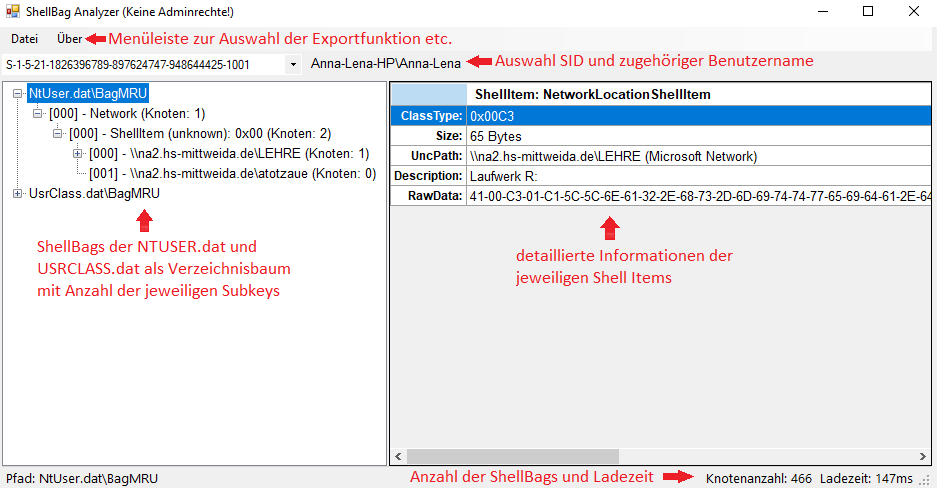
\includegraphics[width=1\textwidth]{part/analyzer.png}
	\caption{Ausschnitt des \glqq ShellBag Analyzers\grqq{}} 
	\label{img:analyzer}
\end{figure}

	
	% Validierung
	\section{Validierung}
Um das implementierte Tool zu testen, wird eine virtuelle Maschine verwendet. Hierfür war es zunächst notwendig, die Virtualisierungssoftware VirtualBox \footnote{Download unter \url{https://www.chip.de/downloads/VirtualBox_23814448.html}, zuletzt verfügbar am 16.04.2020}  herunterzuladen. Im Anschluss war es möglich, bei Microsoft eine bereits fertige virtuelle Maschine (VM) mit Windows 10 als 90 Tage lang kostenlose Version \footnote{Download unter \url{https://developer.microsoft.com/en-us/microsoft-edge/tools/vms/}, zuletzt verfügbar am 16.04.2020}  herunterzuladen. Diese VM kann nach dem Entpacken problemlos in VirtualBox importiert und ausgeführt werden. \\
%welche Einstellungen noch vorgenommen, noch was installiert?, wie das Tool reingebkommen 
\\
Um zu testen, ob das Tool eine korrekte Auswertung der ShellBag-Informationen vornimmt, wird im Folgenden eine Testreihe durchgeführt. Zunächst wurde die SID des aktuell angemeldeten Benutzers mit dem Befehl \glqq \texttt{whoami /user}\grqq{} in der Eingabeaufforderung bestimmt, um im Tool den richtigen Benutzer auszuwählen. Da während der Installation und Konfiguration der virtuellen Maschine bereits ShellBag-Informationen entstanden sind, wurden zunächst die aktuellen ShellBag-Informationen des Benutzers im Tool ausgegeben und in der nachfolgenden Abbildung festgehalten. \\
\\
Basierend auf diesem Ergebnis wurde nun eine Testreihe aufgestellt und eine erneute Auswertung im Tool vergenommen. Die nachfolgende Tabelle \ref{akt} zeigt die durchgeführten Aktivitäten mit den entsprechenden Zeitangaben. Diese Zeiten wurden entsprechend in der Systemsteuerung eingestellt.

\begin{longtable}{|p{0.3\textwidth}|p{0.6\textwidth}|}
	\caption{Testreihe für Ordneraktivitäten} \label{akt} \vspace{1em} \\
	\hline
	\cellcolor{gray!25}\textbf{Zeit} & \cellcolor{gray!25}\textbf{Aktivität} \\
	\hline
	03.06.2020 14:00 Uhr & Anlegen eines Ordners \glqq test\grqq{} \\
	\hline
	03.06.2020 14:05 Uhr & Öffnen und Schließen des Ordners \glqq test\grqq{} \\
	\hline
	04.06.2020 15:00 Uhr & Anlegen eines Ordners \glqq studium\grqq{} \\
	\hline
	04.06.2020 15:10 Uhr & Öffnen und Schließen des Ordners \glqq studium\grqq{} \\
	\hline
	05.06.2020 16:00 Uhr & Anlegen eines Unterordners \glqq softwareprojekt\grqq{} \\
	\hline
	05.06.2020 16:25 Uhr & Öffnen und Schließen des Ordners \glqq softwareprojekt\grqq{} \\
	\hline
	06.06.2020 10:00 Uhr & Standardordner je nachdem (root und volume je) \\
	\hline
\end{longtable}
\vspace{1em}

%Auswertung, ist Unterordner unter Ordner?, stimmen die Informationen wie Zeitstempel etc --> alles abgleichen aus Tabellen, Fehler?, Screenshot zeigen, stimmt Zuordnung Value - Subkey?, kurzes Fazit

%Nun wurde die im Tool integrierte Export-Funktion getestet. Dafür wurden die aus der Testreihe ausgegeben ShellBag-Informationen exportiert. \\
%Test, die Infos zu exportieren mit Screenshot, wie vorgehen, welches Format
%\\
%Im letzten Schritt wurde die Lösch-Funktion des Tools getestet. Dafür wurden die in der Testreihe entstandenen ShellBag-Informationen gelöscht. Im Anschluss wurde der Registrierungs-Editor geöffnet, um zu überprüfen, ob die ShellBag-Informationen des angemeldeten Benutzers unter \texttt{HKU$\backslash$SID\_User$\backslash$Software$\backslash$Classes$\backslash$Local Settings$\backslash$Software$\backslash$Microsoft$\backslash$Windows$\backslash$Shell$\backslash$BagMRU} tatsächlich entfernt wurden.

%Test, die ShellBags zu löschen, wie vorgehen, evtl Screenshot der Registry
	
	% Diskussion
	\section{Diskussion}
\vspace{0.5cm}
Im Folgenden wird sich mit den Ergebnissen der Arbeit auseinandergesetzt. Es erfolgt eine Auswertung, wie gut das Tool den genannten Qualitätsanforderungen entspricht und welche Verbesserungen hätten vorgenommen werden können.
\subsection{Allgemeines}
\vspace{0.3cm}
Grundlage für die Implementierung des Tools stellt das .NET Framework dar. Dieses hat den Nachteil, dass es ausschließlich auf Windows-Betriebssystemen verfügbar ist und auch in Zukunft keine Weiterentwicklung erfolgen wird \cite{netfw,ende}. Vielmehr ist eine Zusammenführung mehrerer Produktlinien zu .NET 5.0 im November 2020 geplant \cite{ende}. Wenn für das Tool zukünftig noch eine Post-Mortem-Analyse implementiert werden würde, dann wäre es somit nur unter Windows lauffähig. Die quelloffene Entwicklungsplattform .NET Core, mit der ebenfalls Programme entwickelt und ausgeführt werden können, hätte den Vorteil gehabt, dass es neben Windows- auch auf Linux- und macOS-Betriebssystemen verfügbar gewesen wäre und somit die ShellBags offline auch auf diesen Systemen hätten untersucht werden können \cite{netcore}. Der Nachteil hierbei ist jedoch, dass der Windows Forms Designer, welcher der Erstellung der grafischen Benutzeroberfläche dient, bisher nur in einer Preview-Version vorliegt, was die Erstellung einer GUI erschweren würde \cite{preview}. So zum Beispiel wird das DataGridView-Steuerelement, welches der tabellarischen Anzeige von Daten dient, hier noch nicht unterstützt, was somit die Nutzung von .NET Core bisher nicht ermöglicht \cite{datagrid,dient}. Aus diesem Grund wurde auf das .NET Framework zurückgegriffen. Es ist jedoch denkbar, dass bei vollständiger Entwicklung eine Portierung vom .NET Framework zu .NET Core oder .NET 5.0 durchgeführt wird \cite{port}.

Weiterhin bleibt festzuhalten, dass die Auswertung der ShellBag-Informationen auf bereits geprüften Erkenntnissen basiert. So erfolgte eine Auswertung der File Entry-, Root Folder- sowie Volume Shell Items, deren Struktur bereits im Rahmen der Bachelorarbeit von Anna-Lena Totzauer untersucht wurde \cite{ba}. Darüber hinaus erlangte man aufgrund der vorliegenden ShellBag-Informationen von Conny Karras die Erkenntnis, dass ShellBags von sogenannten Shared Folders mit dem Class Type Indicator von 0xC3 unter \texttt{HKU$\backslash$SID\_User$\backslash$Software$\backslash$Micro- \newline soft$\backslash$Windows$\backslash$Shell$\backslash$BagMRU}, also in der NTUSER.dat abgelegt werden. Dieser Class Type Indicator wurde nach Joachim Metz auch schon gesichtet und in die Gruppe der Network Location Shell Items eingeordnet. Nach Metz existieren noch weitere Arten von Shell Items. Diese wurden jedoch bisher nicht analysiert, weshalb auf eine Einbeziehung in das selbst implementierte Tool aufgrund der fehlenden Überprüfung auf Korrektheit verzichtet wurde. Es ist jedoch durchaus denkbar, das Tool in Zukunft zu erweitern, sofern die Aussagen von Joachim Metz belegt werden können. Außerdem wurde davon ausgegangen, dass Root Folder Shell Items eine Größe von 20 Byte besitzen, um zu vermeiden, dass Shell Items mit dem Class Type Indicator von 0x1F mit einer anderen Struktur fehlerhaft der Kategorie der Root Folder Shell Items zugeordnet werden, obwohl dies gar nicht der Fall ist. \cite{shelltype}

Außerdem bleibt anzumerken, dass dieses Tool eine forensische Analyse der ShellBag-Infor- \newline mationen eines Windows 10 Betriebssystems ermöglicht. Wie bereits in der Bachelorarbeit von Anna-Lena Totzauer herausgefunden wurde, existieren durchaus Unterschiede zwischen den verschiedenen Betriebssystemen. Es ist somit denkbar, das Tool zukünftig auch für andere Windows-Betriebssysteme zu erweitern. \cite{ba,lo2014windows}

\subsection{Abgleich mit den Qualitätsanforderungen}
\vspace{0.3cm}
Nachfolgend wird diskutiert, ob das Tool die in Kapitel \ref{quali} genannten Qualitätsanforderungen erfüllen konnte.

\paragraph{Kompatibilität:}
Bezüglich der Kompatibilität des Tools konnten die Anforderungen erfüllt werden. Aufgrund der Nutzung des .NET Frameworks ist eine ShellBag-Live-Analyse ausschließlich auf Windows-Systemen, speziell unter Windows 10, möglich.

\paragraph{Integrität:}
Wie sich bei der Validierung des Tools herausstellte, wurden alle ShellBag-Einträge aus der Registry korrekt und vollständig in das Tool übertragen, weshalb hierbei eine Integrität sichergestellt werden kann. Auch die hierarchische Struktur der Einträge konnte beibehalten werden. Im Exportmodus blieb die hierarchische Struktur der ShellBags ebenfalls erhalten und es erfolgten zudem auch keine Manipulationen. Alle Einträge wurden vollständig übernommen, weshalb auch diese Anforderung erfüllt werden kann.

\paragraph{Zuverlässigkeit:}
Grundsätzlich arbeitet das Tool zuverlässig. Grundlegende Fehlermeldungen werden im Programm abgefangen. Ist beispielsweise ein Zeitstempel im Value eines File Entry Shell Items inkorrekt oder ungültig, so wird dieser Fehler abgefangen und dem Zeitstempel der Wert null zugewiesen. Somit wird vermieden, dass im Tool falsche Informationen ausgegeben werden. Ein eventueller Absturz des Tools kann jedoch nicht ausgeschlossen werden, da auch unvorhersehbare Fehler auftreten können, welche bisher nicht vom Programm abgefangen werden. In diesem Fall sollte eine Optimierung des Quellcodes stattfinden.

\paragraph{Benutzerfreundlichkeit:}
Das Tool ermöglicht mit Hilfe der Bedienungsanleitung einen leichten Einstieg für den Nutzer. Es wurde schlicht und benutzerfreundlich gestaltet. Alle Voraussetzungen zum Betrieb sowie Auswahlmöglichkeiten im Tool wurden in der Bedienungsanleitung erläutert.

\paragraph{Leistungseffizienz:}
Die Leistungseffizienz kann anhand der im Tool ausgegebenen Ladezeit bewertet werden. Die Zeit beschreibt die Dauer, welche das Tool benötigte, um die ShellBag-Informationen aus der Registry auszuwerten. Diese Zeit führte zu einem zufriedenstellenden Ergebnis, denn 7 ShellBag-Einträge konnten innerhalb von 20 ms ausgewertet werden, das entspricht im Schnitt 2,86 ms pro ShellBag-Eintrag. Bei Tests im Verlauf der Arbeit konnten teilweise sogar noch geringere Ladezeiten pro ShellBag-Eintrag festgestellt werden. Dies ist immer abhängig davon, wie viele Prozesse parallel laufen.

\paragraph{Portabilität:}
Wie in der Validierungsphase festgestellt werden konnte, war eine schnelle Portierung zwischen dem Host- und Gastsystem in einer VM möglich. Das Tool war sofort einsatzbereit. Die einzige Voraussetzung ist die Installation des .NET Frameworks 4.8.


	
	% Ergebnisse und Diskussion
	\section{Fazit}
...
%durch .net framework nur für windows möglich

	% Ausblick
	\section{Ausblick}
\vspace{0.5cm}
In Zukunft wäre es denkbar, eine Portierung vom .NET Framework auf .NET Core oder .NET 5.0 vorzunehmen. Dies würde die Möglichkeit eröffnen, neben der Live-Analyse auch eine Post-Mortem-Analyse der Windows-ShellBags zu implementieren, deren Auswertung neben Windows- auch auf Linux- oder macOS-Betriebssystemen möglich wäre. Der Vorteil davon wäre somit, dass das Tool eine höhere Kompatibilität aufweist und auf verschiedenen Betriebssystemen lauffähig ist, je nachdem welches Betriebssystem die forensische Workstation besitzt. \cite{netcore,port} \\
\\
Weiterhin existieren neben File Entry-, Root Folder-, Volume- und Network Location Shell Items noch andere Arten. In der vorliegenden Arbeit wurden nur die bereits geprüften Erkenntnisse in der Auswertung der ShellBags berücksichtigt. Das Tool sollte daher zukünftig erweitert werden, sofern beispielweise die Informationen von Joachim Metz bezüglich Shell Items bestätigt werden. Auch vor allem die ShellBags in der NTUSER.dat haben noch ein großes Analysepotenzial. \cite{shelltype} \\
\\
Außerdem dient das Tool bisher einer forensischen Analyse der ShellBags eines Windows 10 Betriebssystems. Da jedoch Unterschiede zwischen den einzelnen Betriebssystemen existieren, sollte das Tool zukünftig auch um die anderen Betriebssystemversionen erweitert werden, um die Anwendungsfähigkeit des Tools zu erweitern. \cite{ba}


	\newpage
	% Literatur
	\bibliographystyle{alpha}
	\bibliography{Literatur}
	\addcontentsline{toc}{section}{Literaturverzeichnis}
	
	\newpage
	\thispagestyle{empty}
	\section*{Selbstständigkeitserklärung}
	\vspace{15mm}
	
	Hiermit erkläre ich, dass ich die vorliegende Arbeit selbstständig und nur unter Verwendung der angegebenen
	Quellen und Hilfsmittel angefertigt habe. Sämtliche Stellen der Arbeit, die im Wortlaut oder dem Sinn nach
	Publikationen oder Vorträgen anderer Autoren entnommen sind, habe ich als solche kenntlich gemacht. Diese
	Arbeit wurde in gleicher oder ähnlicher Form noch keiner anderen Prüfungsbehörde vorgelegt oder anderweitig
	veröffentlicht.
	
	\vspace{2cm}
	
	\begin{tabular}{lp{2em}l}
		\hspace{4cm} && \hspace{7cm} \\ \cline{1-1}\cline{3-3} \\
		Ort, Datum && Unterschrift
	\end{tabular}
	\vspace{1cm}

	\begin{tabular}{lp{2em}l}
	\hspace{4cm} && \hspace{7cm} \\ \cline{1-1}\cline{3-3} \\
	Ort, Datum && Unterschrift
	\end{tabular}

\end{document}
